\documentclass[acmsmall,review,anonymous]{acmart}

%\settopmatter{printfolios=true,printccs=false,printacmref=false}

%% NOTES among authors 
\def\notes#1{\expandafter\def\csname#1\endcsname##1{\marginpar{\par\noindent\hrulefill\par\raggedright\tiny\noindent #1: ##1}}}
% \def\notes#1{\expandafter\def\csname#1\endcsname##1{\marginpar{\relax}}}
\notes{bg}
\notes{cd}
\notes{mf}

\overfullrule=1mm
\citestyle{acmauthoryear}
%\setcitestyle{round}

\usepackage{alltt}
\usepackage{amssymb}
\usepackage{calc}
\usepackage{listings}
\usepackage{mathpartir}
\usepackage{pifont}
\usepackage{tikz}
\usepackage{wrapfig}
\usepackage{xcolor}
\usetikzlibrary{shapes.geometric}

\begin{document}

\title{Exploring the Deeps and Shallows: A Rational Programmer Study of How Various Profilers Can Guide 3D Type Migration}

\author{Ben Greenman}
\orcid{0000-0001-7078-9287}
\affiliation{%
  \institution{PLT @ Brown University}
  \city{Providence}
  \state{Rhode Island}
  \country{USA}
}
\email{benjaminlgreenman@gmail.com}

\author{Matthias Felleisen}
\orcid{0000-0001-6678-1004}
\affiliation{%
  \institution{PLT @ Northeastern University}
  \city{Boston}
  \state{Massachusetts}
  \country{USA}
}
\email{matthias@ccs.neu.edu}

\author{Christos Dimoulas}
\orcid{0000-0002-9338-7034}
\affiliation{%
  \institution{PLT @ Northwestern University}
  \city{Evanston}
  \state{Illinois}
  \country{USA}
}
\email{chrdimo@northwestern.edu}

%\renewcommand{\shortauthors}{...}

%%
%% The abstract is a short summary of the work to be presented in the
%% article.
\begin{abstract}
  TBD
\end{abstract}


%%
%% The code below is generated by the tool at http://dl.acm.org/ccs.cfm.
%% Please copy and paste the code instead of the example below.

\begin{CCSXML}
<ccs2012>
<concept>
<concept_id>10011007.10011006.10011039.10011311</concept_id>
<concept_desc>Software and its engineering~Semantics</concept_desc>
<concept_significance>500</concept_significance>
</concept>
<concept>
<concept_id>10011007.10011006.10011008.10011024.10011032</concept_id>
<concept_desc>Software and its engineering~Constraints</concept_desc>
<concept_significance>100</concept_significance>
</concept>
<concept>
<concept_id>10011007.10011006.10011008.10011009.10011012</concept_id>
<concept_desc>Software and its engineering~Functional languages</concept_desc>
<concept_significance>100</concept_significance>
</concept>
</ccs2012>

\end{CCSXML}

\ccsdesc[500]{Software and its engineering~Semantics}
\ccsdesc[100]{Software and its engineering~Constraints}
\ccsdesc[100]{Software and its engineering~Functional languages}

\keywords{complete monitoring, blame soundness, blame completeness}

\maketitle

\section{Introduction}
\label{s:introduction}

Rational programmer~\cite{lgfd-icfp-2021}.


\section{Results}
\label{s:data}

\begin{table}[t]
  \caption{Out of all configurations, how many improve to under 2x after switching all typed configs to D or to S?
  Does not count no-ops.}
  \label{t:micros}
  \begin{tabular}{lrr}
    Benchmark & All-D & All-S \\\midrule
    sieve & 33.33\% & 11.11\% \\
    forth & 13.58\% & 7.41\% \\
    morsecode & & \\
    fsm & 45.68\% & 11.11\% \\
    fsmoo & 45.68\% & 0.00\% \\
    kcfa & 30.00\% & 58.02\% \\
    jpeg & 43.21\% & 46.91\% \\
    lnm & 72.15\% & 23.05\% \\
    snake & 9.69\% & 0.26\% \\
    take5 & 19.88\% & 2.56\% \\
    acquire & 20.13\% & 46.32\% \\
    tetris & 32.17\% & 7.60\% \\
    synth & 5.86\% & 21.84\% \\
  \end{tabular}

\end{table}

\begin{figure}[t]
  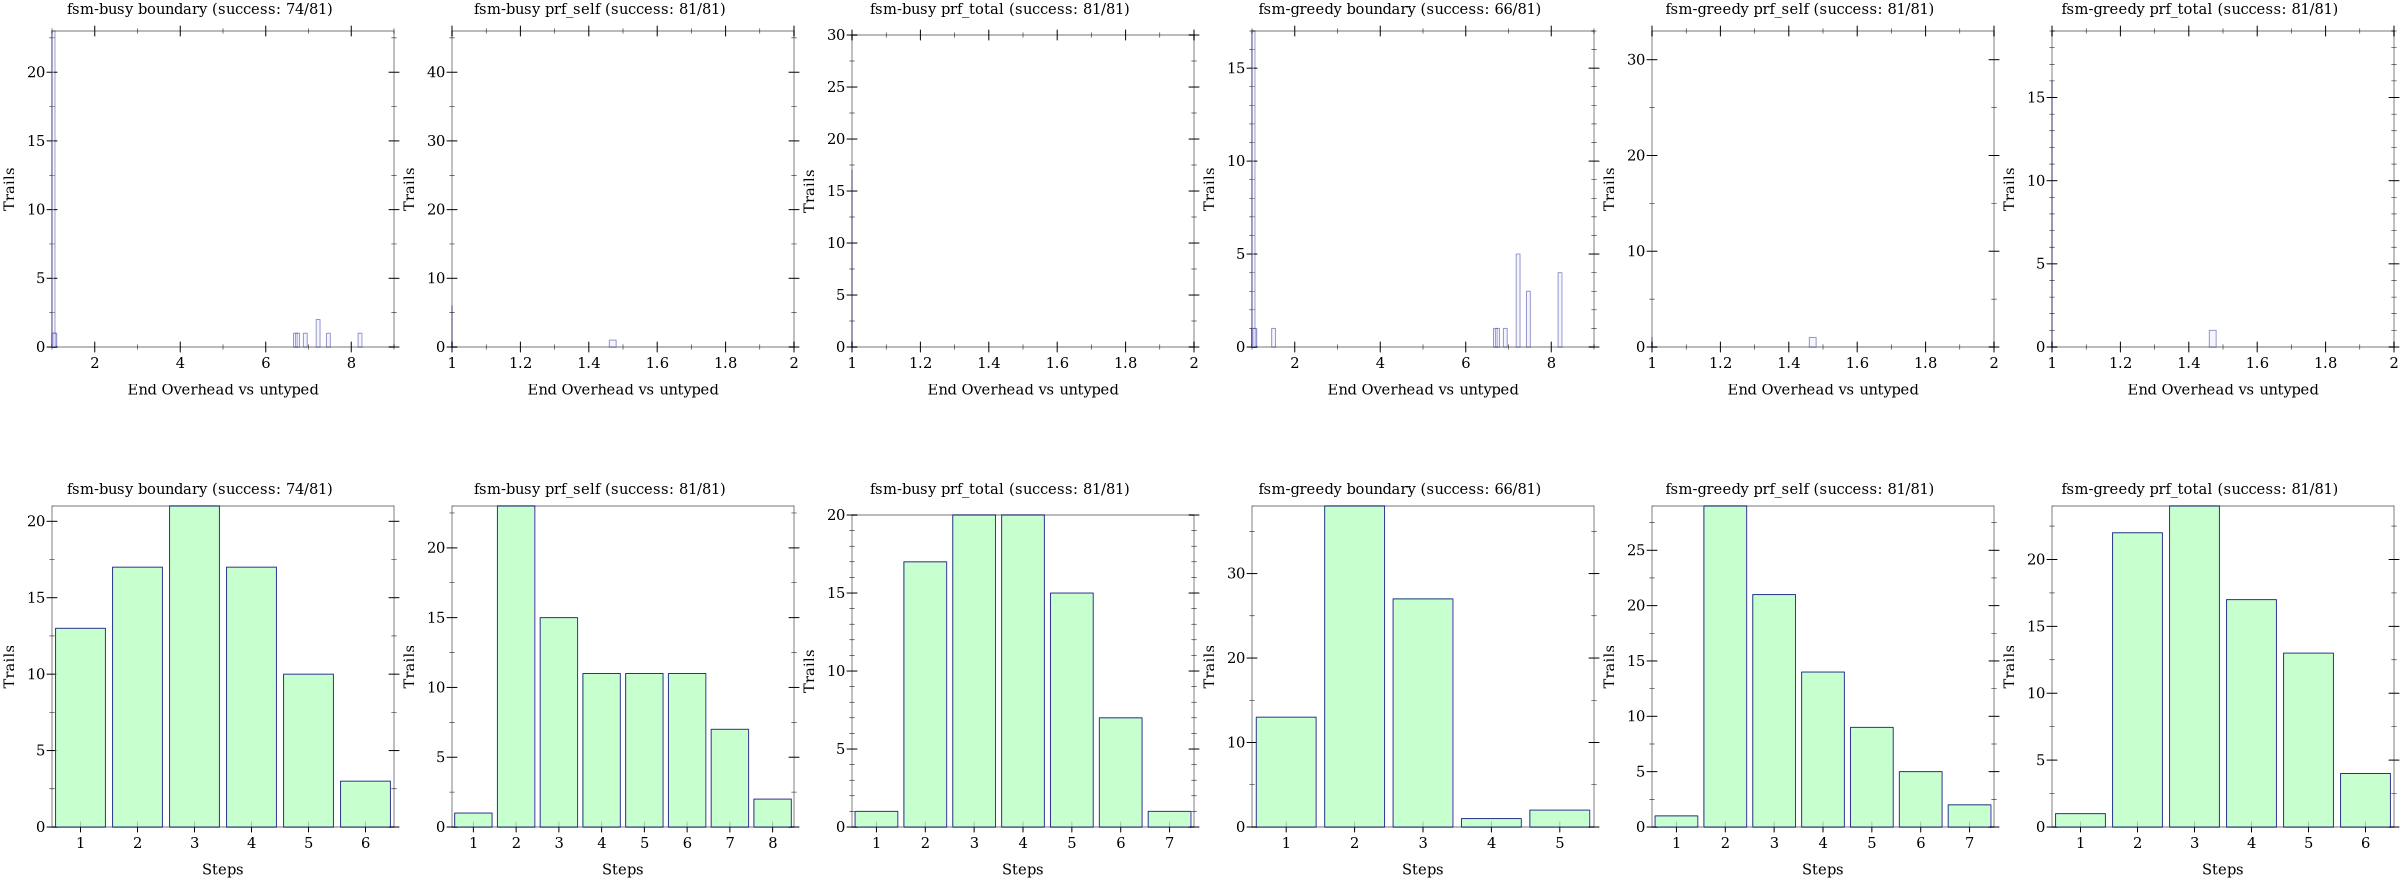
\includegraphics[width=\columnwidth]{img/sample.png}
  \caption{FSM outcomes}
  \label{f:sample}
\end{figure}


\section{Discussion}
\label{s:conclusion}
\label{s:discussion}



\begin{acks}
  TBD

We gratefully acknowledge support from
  \grantsponsor{NSF}{NSF}{https://www.nsf.gov}
 grants
  (?) \href{"https://www.nsf.gov/awardsearch/showAward?AWD_ID=1763922"}{\grantnum{NSF}{CCF 1763922}},
  (?) \href{"https://www.nsf.gov/awardsearch/showAward?AWD_ID=1823244"}{\grantnum{NSF}{CNS 1823244}},
 and
 \href{"https://www.nsf.gov/awardsearch/showAward?AWD_ID=2030859"}{\grantnum{NSF}{CCF 2030859}}
  to the CRA for the \href{https://cifellows2020.org}{CIFellows} project.
\end{acks}

\bibliographystyle{ACM-Reference-Format}
\bibliography{bib}

\end{document}
\endinput
